\documentclass[12pt,a4paper,twoside,openright,titlepage,final]{article}
\usepackage{fontspec}
\usepackage{amsmath}
\usepackage{amsfonts}
\usepackage{amssymb}
\usepackage{makeidx}
\usepackage{graphicx}
\usepackage[hidelinks,unicode=true]{hyperref}
\usepackage[spanish,es-nodecimaldot,es-lcroman,es-tabla,es-noshorthands]{babel}
\usepackage[left=3cm,right=2cm, bottom=4cm]{geometry}
\usepackage{natbib}
\usepackage{microtype}
\usepackage{ifdraft}
\usepackage{verbatim}
\usepackage[nottoc]{tocbibind}
\usepackage{pdflscape}
\usepackage[obeyDraft]{todonotes}
\ifdraft{
	\usepackage{draftwatermark}
	\SetWatermarkText{BORRADOR}
	\SetWatermarkScale{0.7}
	\SetWatermarkColor{red}
}{}
\usepackage{booktabs}
\usepackage{longtable}
\usepackage{calc}
\usepackage{array}
\usepackage{caption}
\usepackage{subfigure}
\usepackage{footnote}
\usepackage{url}
\usepackage[titletoc]{appendix}

\setsansfont[Ligatures=TeX]{texgyreadventor}
\setmainfont[Ligatures=TeX]{texgyrepagella}
\setmonofont{FreeMono}

\usetikzlibrary{decorations.pathreplacing}

%*******************************************************
%                 NO MODIFICAR
\newcommand*{\FSfont}[1]{%
  \fontencoding{T1}\fontfamily{#1}\selectfont}

\newlength{\tpheight}\setlength{\tpheight}{0.9\textheight}
\newlength{\txtheight}\setlength{\txtheight}{0.9\tpheight}
\newlength{\tpwidth}\setlength{\tpwidth}{0.9\textwidth}
\newlength{\txtwidth}\setlength{\txtwidth}{0.9\tpwidth}
\newlength{\drop}
%*******************************************************

% Crea una portada con los siguientes parámetros
%
% #1 : Título 
% #2 : Subtítulo
% #3 : Subsubtítulo
% #4 : Autor(es)
% #5 : Lugar
%

\newcommand*{\portada}[5]{
\begin{titlepage}
\begingroup
\vspace*{1cm}
\drop = 0.2\txtheight
\centering
\vfill
{\Huge \scshape #1}\\[\baselineskip]
{\Large \textbf{#2}}\\[\baselineskip]
{\Large \scshape #3}\\[\baselineskip]
\vspace*{0.3cm}
{\large \textit{#4}}\\[0.5\drop]

\includegraphics[scale=0.35]{./imagenes/logoURJC.jpg}
\vspace*{1.5cm}

{\large \scshape #5, \today} \par
\begin{center}
\end{center}
\vfill\null
\endgroup
\end{titlepage}
}
 %*****************************************************
 


\author{José Ignacio Escribano}

\title{}

\setlength{\parindent}{0pt}

\begin{document}

\pagenumbering{alph}
\setcounter{page}{1}

\portada{Caso Práctico II}{Minería de datos}{Estimación y predicción con redes neuronales}{José Ignacio Escribano}{Móstoles}

\listoffigures
\thispagestyle{empty}
\newpage

\tableofcontents
\thispagestyle{empty}
\newpage


\pagenumbering{arabic}
\setcounter{page}{1}

\section{Introducción}

En este caso práctico, pondremos en práctica lo aprendido en teoría sobre redes neuronales, a través de dos librerías distintas de R que las implementan. Éstas son \texttt{nnet} y \texttt{neuralnet}.

\section{Resolución de las cuestiones de evaluación}

A continuación resolveremos las cuestiones planteadas en el caso práctico. En todas las cuestiones de evaluación consideraremos la función no lineal dada por $y = x \sin x$ en el intervalo $[-2\pi, 2\pi]$.

\subsection{Cuestión 1}
Representamos la función $y = x \sin x$ tomando 200 puntos en el intervalo $[-2\pi, 2\pi]$. La función queda como se muestra en la Figura~\ref{fig:funcion_con_type}.\\

\begin{figure}[tbph!]
\centering
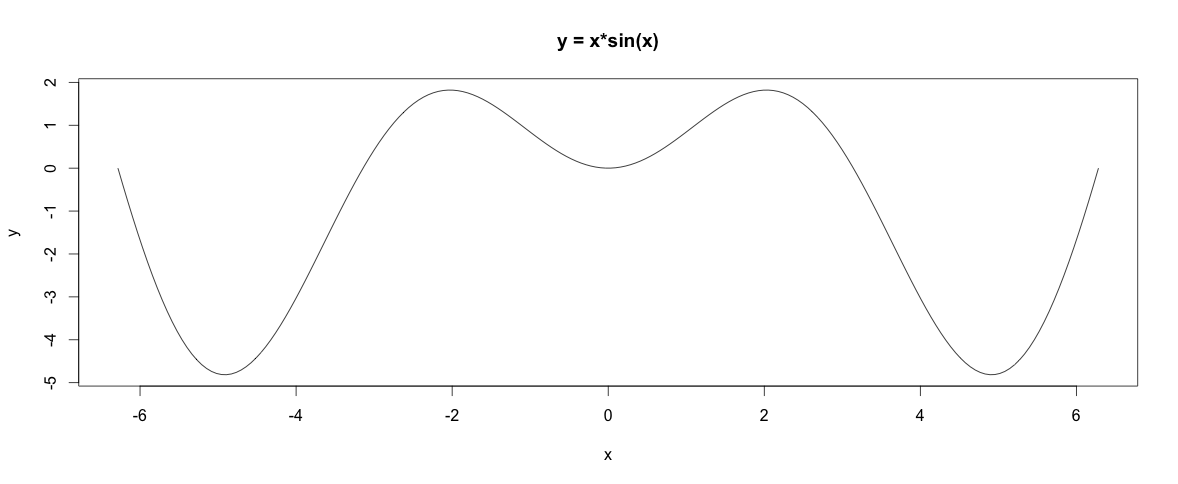
\includegraphics[width=0.8\linewidth]{imagenes/funcion_con_type}
\caption{Función $y = x\sin x$ con 200 puntos}
\label{fig:funcion_con_type}
\end{figure}

Si dibujamos la función sin el parámetro \texttt{type='l'}, tenemos que sólo se muestran los puntos $\{(x_i, x_i \sin x_i)\}$  con $i = 1,\dots, 200$ en el plano. El parámetro \texttt{type='l'} lo que hace es interpolar los dintintos puntos para obtener una curva. La Figura~\ref{fig:funcion_sin_type} muestra este hecho.\\

\begin{figure}[tbph!]
\centering
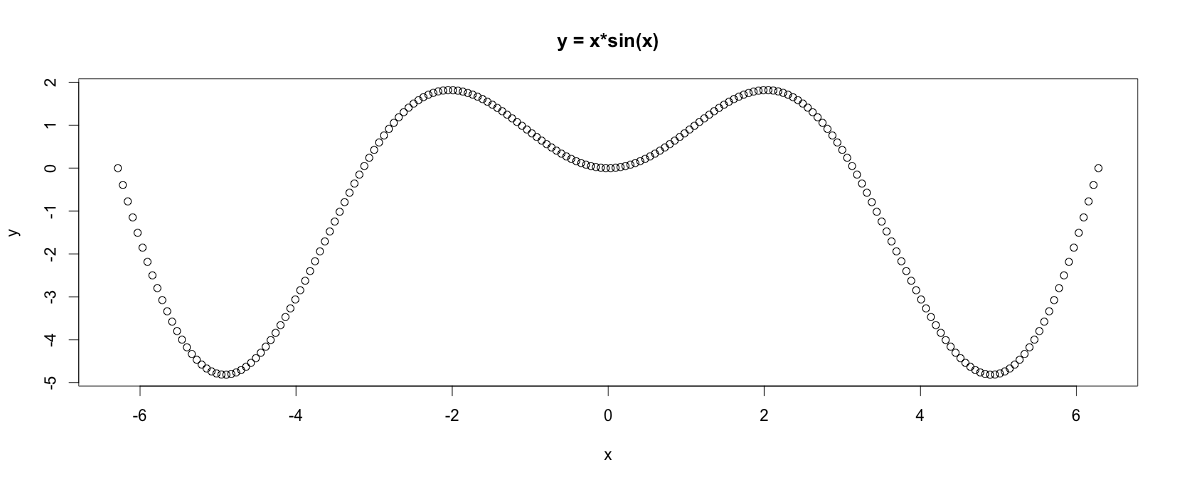
\includegraphics[width=0.8\linewidth]{imagenes/funcion_sin_type}
\caption{Función $y = x\sin x$ con 200 puntos sin el parámetro type='l'}
\label{fig:funcion_sin_type}
\end{figure}

Esta función sí podrá ser aproximada por una red neuronal, ya que aunque se trate de una función no lineal, el Teorema de Cybenko nos asegura que una red neuronal multicapa puede aproximar una función continua en subconjuntos compactos de $\mathbb{R}^n$, que es lo que intentamos aproximar.

\subsection{Cuestión 2}

Ajustamos un modelo lineal con los 200 puntos calculados anteriormente. El resumen que muestra R es el siguiente:

\begin{verbatim}
Call:
lm(formula = y ~ x)

Residuals:
       Min         1Q     Median         3Q        Max 
-3.8188378 -2.2907973  0.9951677  2.0555346  2.8136221 

Coefficients:
              Estimate     Std. Error  t value        Pr(>|t|)    
(Intercept) -0.9946693  0.16374284208 -6.07458 0.0000000062568 ***
x           -0.0000000  0.04491295114  0.00000               1    
---
Signif. codes:  0 ‘***’ 0.001 ‘**’ 0.01 ‘*’ 0.05 ‘.’ 0.1 ‘ ’ 1

Residual standard error: 2.315673 on 198 degrees of freedom
Multiple R-squared:  6.660172e-32,	Adjusted R-squared:  -0.005050505 
F-statistic: 1.318714e-29 on 1 and 198 DF,  p-value: 1
\end{verbatim}

La recta de regresión es $y=-1$. La Figura~\ref{fig:recta} muestra la recta de regresión sobre la función. La Figura indica un ajuste bastante malo. Esto lo corroboramos con el coeficiente de determinación, $R^2$, que es prácticamente 0, por lo que no hay relación lineal entre los valores de x e y.\\ 

\begin{figure}[tbph!]
\centering
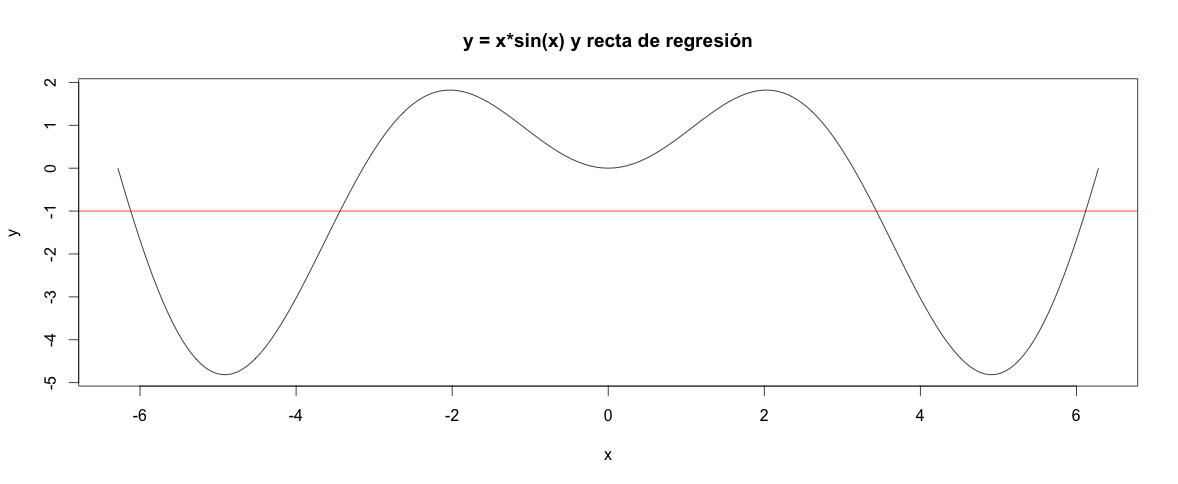
\includegraphics[width=0.8\linewidth]{imagenes/recta}
\caption{Recta de regresión de la función $y=x\sin x$}
\label{fig:recta}
\end{figure}

Comprobemos que se incumplen las hipótesis del modelo: normalidad en los residuos y/o linealidad. Para ello, representamos en R, un Q-Q plot y un gráfico de residuos (Figura~\ref{fig:residuos}).\\

\begin{figure}[htbp!]
\centering
\subfigure[Q-Q plot]{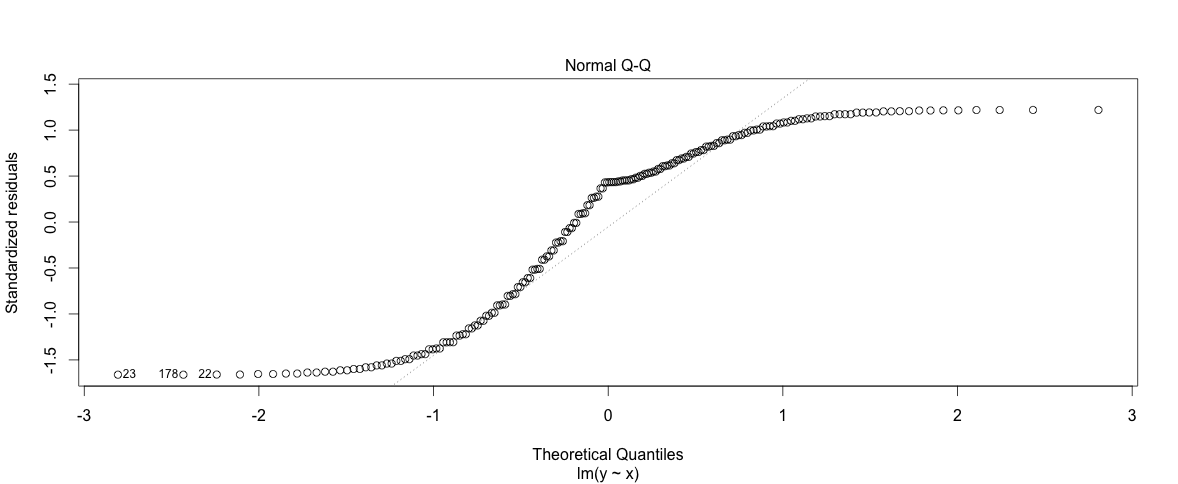
\includegraphics[width=0.80\linewidth]{imagenes/qqplot}}
\subfigure[Residuos]{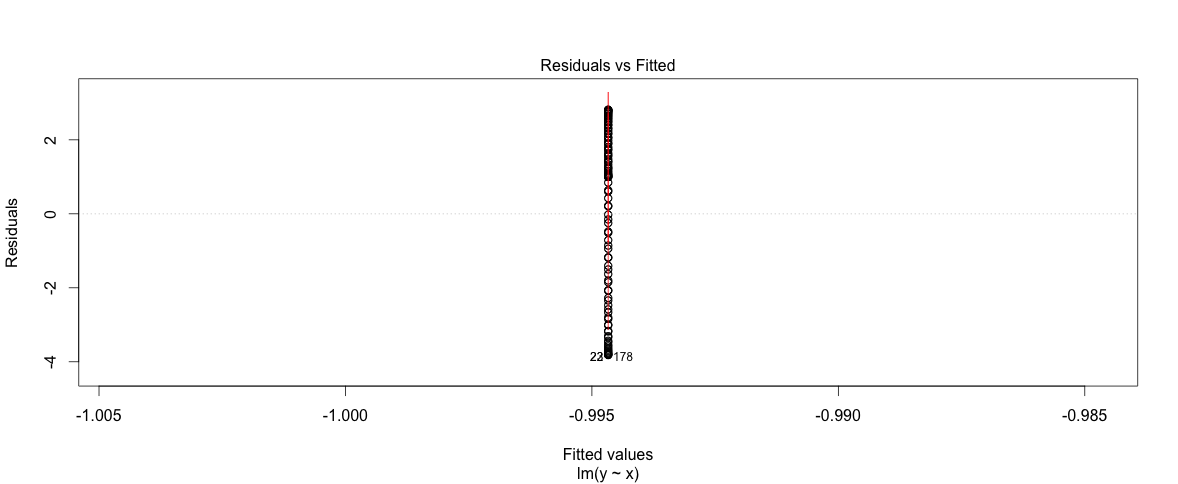
\includegraphics[width=0.80\linewidth]{imagenes/errores}}
\caption{Q-Q plot y gráfico de residuos del modelo lineal} \label{fig:residuos}
\end{figure}

Observamos que los residuos no están normalmente distribuidos, por lo que este modelo no es válido. No hay relación lineal entre los valores de $x$ e $y$.

\subsection{Cuestión 3}

Procedemos a ajustar la función con una red neuronal. Representamos la función original junto con la función de ajuste de la red neuronal desde 1 hasta 10 neuronas (Figura~\ref{fig:diferentes_neuronas}).\\

\begin{figure}[tbph!]
\centering
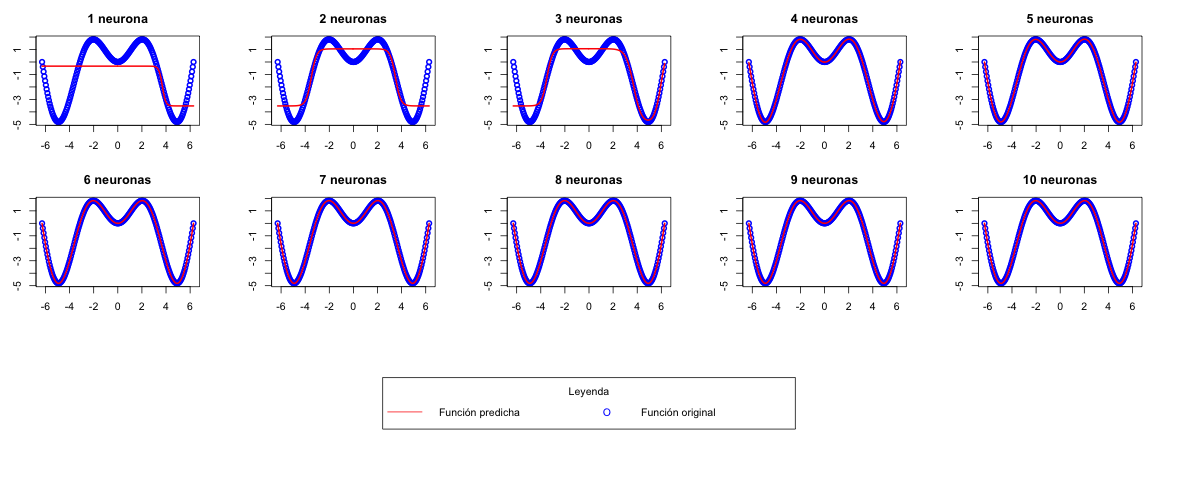
\includegraphics[width=1\linewidth]{imagenes/diferentes_neuronas}
\caption{Predicción con distintas neuronas}
\label{fig:diferentes_neuronas}
\end{figure}

Se observa que, a medida que aumentamos el número de neuronas, el ajuste de la función aprendida cada vez es mejor, aunque a partir de la cuarta neurona, apenas hay diferencias entre entre la función predicha y la original. Por tanto, con 4 neuronas es suficiente para predecir correctamente esta función.\\

A modo de ejemplo, vemos la salida que produce R para la red con 4 neuronas.

\begin{verbatim}
# weights:  13
initial  value 1300.296952 
iter  10 value 238.577267
iter  20 value 165.124118
iter  30 value 145.364713
iter  40 value 140.272616
iter  50 value 129.336562
iter  60 value 108.238405
iter  70 value 98.038065
iter  80 value 73.135425
iter  90 value 53.622029
...
iter1200 value 0.336774
iter1210 value 0.335452
iter1220 value 0.327588
iter1230 value 0.326635
iter1240 value 0.318003
final  value 0.317111 
converged
\end{verbatim}

Es decir, converge tras 1240 iteraciones del algoritmo con un error de 0.317111.\\

Por último, representamos la red para 1 y 3 neuronas. Éstas se pueden ver en la Figura~\ref{fig:representacion_red}.\\

\begin{figure}[htbp!]
\centering
\subfigure[1 neurona]{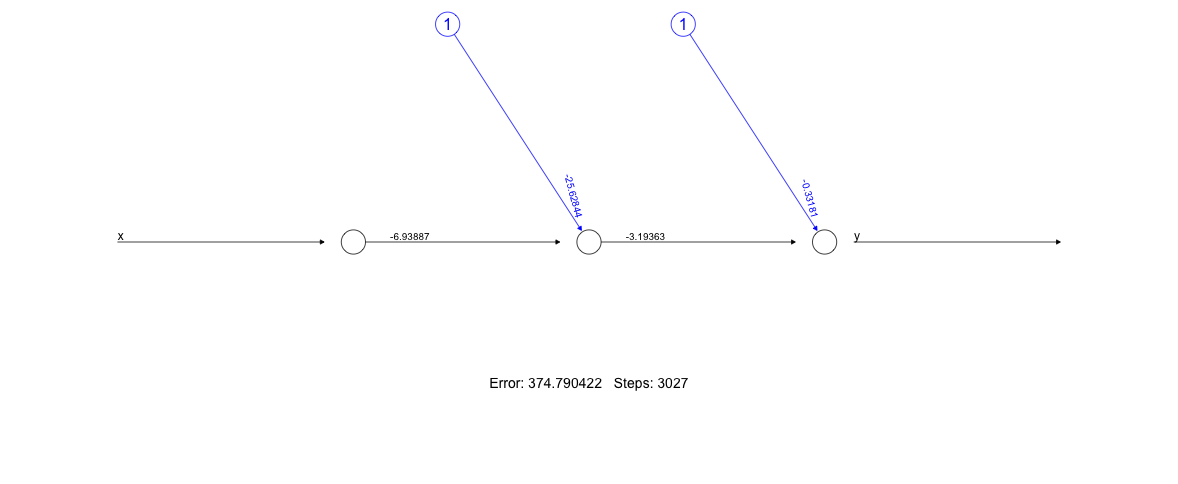
\includegraphics[width=0.80\linewidth]{imagenes/1neurona}}
\subfigure[3 neuronas]{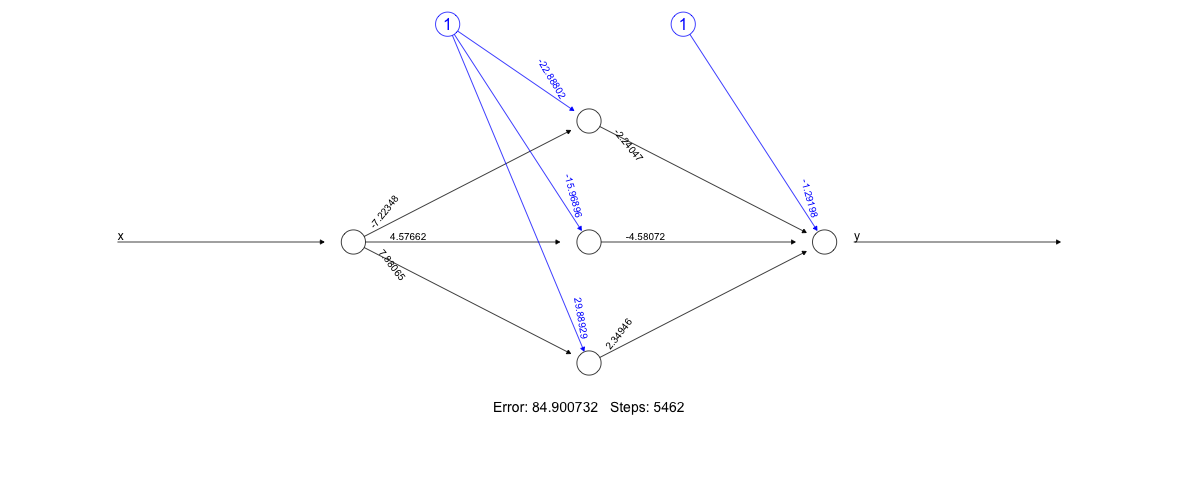
\includegraphics[width=0.80\linewidth]{imagenes/3neuronas}}
\caption{Representación de la red para 1 y 3 neuronas} \label{fig:representacion_red}
\end{figure}

Observamos que, en el caso de una sola neurona tenemos un error de 374.79 tras 3027 iteraciones del algoritmo. En el caso de tres neuronas, tenemos un error de 54.90 tras 5462 iteraciones del algoritmo. De nuevo, vemos que aumentando el número de neuronas de la capa oculta, reducimos el error del ajuste de la función. Notar que se obtienen errores sensiblemente diferentes según se emplee una librería u otra. Esto puede ser debido a la implementación o la inicialización de los pesos del algoritmo utilizado.


\section{Conclusiones}

En este caso práctico, hemos puesto en práctica las redes neuronales para aprender y predecir valores de una función. También hemos visto que es indiferente que la función sea o no lineal, puesto que una red neuronal multicapa será capaz de aprenderla gracias al teorema de Cybenko (sobre un subconjunto compacto de $\mathbb{R}^n$).\\

En R existen distintas librerías que implementan redes neuronales, por lo que hay que tener cuidado a la hora de aplicar una librería u otra ya que pueden variar sensiblemente los resultados según una u otra. Pero conociendo las ventajas de cada librería podremos conseguir grandes resultados gracias a la gran capacidad de cálculo de R.

\clearpage

\section{Código R utilizado}

El código utilizado para la resolución de este caso práctico, separado por cuestiones, se puede ver a continuación:\\

\verbatiminput{caso_2.R}
 

\end{document}